\subsubsection{Prospetto Orario}
La tabella seguente riporta il totale delle ore di lavoro svolte dai singoli membri del gruppo nell'intera durata del progetto, inclusi i periodi di Analisi e di Consolidamento dei requisiti, che non sono infatti rendicontati. La ridistribuzione oraria effettuata nei diversi periodi é stata sempre effettuata puntando a mantenere una distribuzione di lavoro equa tra tutti i componenti del gruppo.

\rowcolors{2}{lightRowColor}{darkRowColor}
\begin{longtable}{
  >{\centering}p{0.20\textwidth}
  >{\centering}p{0.09\textwidth}
  >{\centering}p{0.09\textwidth}
  >{\centering}p{0.09\textwidth}
  >{\centering}p{0.09\textwidth}
  >{\centering}p{0.09\textwidth}
  >{\centering}p{0.09\textwidth}
  >{\centering\arraybackslash}p{0.065\textwidth} }

  \coloredTableHead
  \textbf{\color{white}Nome} &
  \textbf{\color{white}Rp} &
  \textbf{\color{white}As} &
  \textbf{\color{white}An} &
  \textbf{\color{white}Pt} &
  \textbf{\color{white}Pr} &
  \textbf{\color{white}Vf} &
  \textbf{\color{white}Totale}
  \tabularnewline
  \endhead

  % Contenuto della tabella
  % Nome & Rp & As & An & Pt & Pr & Vf & Totale \\
  \VB & 7  & 3 (-1)  & 2 (+2)  & 18 (-1)  & 33 (-1)  & 38       & 101 (-1) \\
  \LB & 5  & 5 (-1)  & 10      & 27 (+1)  & 34 (-1)  & 21 (+1)  & 102 \\
  \NF & 5  & 7 (-1)  & 6       & 27       & 26       & 30       & 101 (-1) \\
  \EG & 6  & 5       & 7       & 30       & 26       & 28       & 102 \\
  \FJ & 11 & 16 (-1) & 2 (+1)  & 18       & 31       & 25       & 102 \\
  \MP & 10 & 13 (-1) & 1 (+1)  & 23       & 22       & 33       & 102 \\
  \AS & 6  & 9 (-1)  & 0 (+1)  & 21       & 31       & 34       & 102 \\
  \AZ & 7  & 8 (-1)  & 10      & 15 (+1)  & 33 (-1)  & 28       & 101 (-1) \\
  \textbf{Ore totali per ruolo} & \textbf{57} & \textbf{66} & \textbf{38} & \textbf{179} & \textbf{236} & \textbf{237} & \textbf{813}  \\
  \textbf{Delta} & \textbf{+0} & \textbf{-7} & \textbf{+5} & \textbf{+1} & \textbf{-3} & \textbf{+1} & \textbf{-3} \\

  \rowcolor{white}\caption {Distribuzione delle ore di investimento e rendicontate complessive}	\\

\end{longtable}
Il grafico sottostante evidenzia le differenze tra il preventivo ed il consuntivo finale rendicontato per ogni membro del gruppo.
% Grafico
Rappresentazione grafica della distribuzione dei ruoli:
\begin{figure}[h]
  \centering
  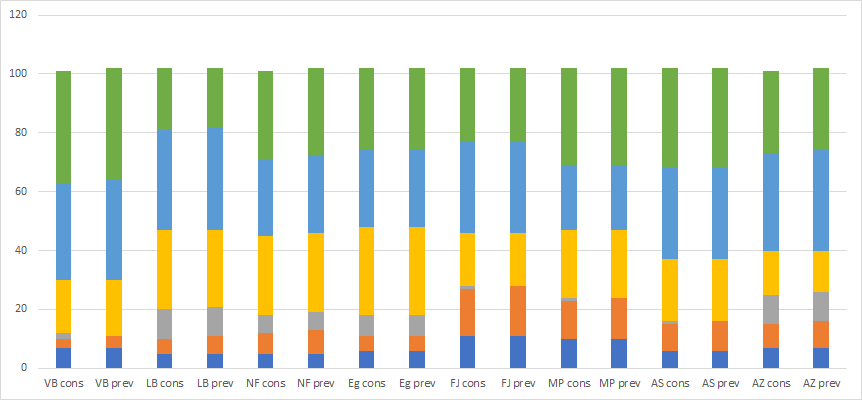
\includegraphics[width=1\textwidth]{./res/img/membro_cons_vs_prev.png}
  \caption{Ripartizione delle ore per ogni ruolo, confrontata tra il preventivo e il
consuntivo finale rendicontato}
\end{figure}

\subsubsection{Prospetto Economico}
Nella seguente tabella si riportano i costi derivati dalle ore impiegate per ogni ruolo durante lo sviluppo del progetto, incluse le fasi di Analisi e di Consolidamento dei requisiti, che non sono rendicontate.

\rowcolors{2}{lightRowColor}{darkRowColor}
\begin{longtable}{
  >{\centering}p{0.25\textwidth}
  >{\centering}p{0.05\textwidth}
  >{\centering\arraybackslash}p{0.15\textwidth} }

  \coloredTableHead
  \textbf{\color{white}Ruolo} &
  \textbf{\color{white}Ore} &
  \textbf{\color{white}Costo in \euro{}}
  \tabularnewline
  \endhead

  % Contenuto della tabella
  % Ruolo & Ore & Costo in \\
  Responsabile    & 57   & 1.710,00 \\
  Amministratore  & 66   & 1.320,00 \\
  Analista        & 38   & 950,00 \\
  Progettista     & 179  & 3.938,00 \\
  Programmatore   & 236  & 3.540,00 \\
  Verificatore    & 237  & 3.555,00 \\
  \textbf{Totale} & \textbf{1102} & \textbf{15.013,00} \\
  \textbf{Totale} & \textbf{-3} & \textbf{-23,00} \\

  \rowcolor{white}\caption {Prospetto dei costi totali delle ore complessive di investimento e rendicontate per ciascun ruolo} \\

\end{longtable}
Dal grafico sottostante si notano le piccole differenze tra preventivo e consuntivo riguardo ogni ruolo di progetto.
% Grafico
Rappresentazione grafica della distribuzione dei ruoli:
\begin{figure}[h!]
  \centering
  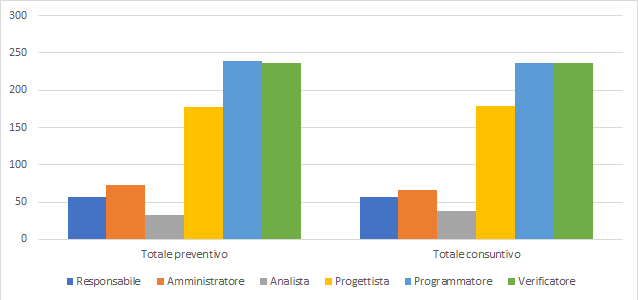
\includegraphics[width=0.9\textwidth]{./res/img/consfinale_vs_prev.png}
  \caption{Ripartizione delle ore per membro del gruppo su ciascun ruolo, con confronto tra il preventivo
e il consuntivo}
\end{figure}

\subsubsection{Conclusioni}
La produzione di una pianificazione coerente e realistica é stata un' attivitá nella quale il grupo ha incontrato diversi ostacoli. I membri del gruppo, non essendo abituati ad organizzare attivitá e compiti in un progetto cosí complesso, hanno prodotto\ped{\textit{G}} una pianificazione piú volte incoerente rispetto al modello di sviluppo dichiarato. Di conseguenza il Responsabile di Progetto e gli Amministratori sono stati portati a dover rivedere piú volte la pianificazione a scopo correttivo. Riuscire da subito a produrre un'ottima pianificazione viene sia dall'esperienza che dalla conoscenza approfondita del prodotto\ped{\textit{G}} da sviluppare.\\
In generale il gruppo è riuscito a rispettare la pianificazione, nonostante delle variazioni nella distribuzione delle ore pianificate all'interno dei diversi periodi ed incrementi. Questi scostamenti dal numero di ore pianificate per i singoli ruoli, sono stati bilanciati grazie ad una ridistribuzione delle ore all'interno dei periodi e non si é mai trattato di oscillazioni considerevoli, rimanendo sotto alle 10 ore per ruolo. Inoltre l'impegno orario é sempre stato distribuito equamente tra i membri del gruppo, evitando di sovraccaricare la singola risorsa.\\
In conclusione, il gruppo riconosce gli errori fatti nella produzione della pianificazione ed evidenziati nei commenti fatti dal Committente, ritenendoli utili all'esperienza formativa.
\newline
\newline
Il gruppo chiude le attività di progetto con un bilancio positivo: 15.013,00 \euro{} totali a fronte di un preventivo di 15.036,00 \euro{}.
